\chapter{System Implementation}
\label{Ch-5:Sec:System}

In this chapter, we will combine the work of Chapter~\ref{Ch-2:Sec:Standardize} and Chapter~\ref{Ch-3:Sec:Extraction}. A data visualization task also includes in this chapter. 

\section{Architecture of System}
\vspace{-5pt}
The flow chart Figure~\ref{fig:section5-pic1} illustrates the frame of whole project. The Q \& A system is separated in three parts:
\begin{enumerate}
	\item Data Processing, including data crawling, data cleaning, data storing and data standardizing, referring to the work in Chapter~\ref{Ch-2:Sec:Standardize}.
	\item Search Engine, including subgraph generating, natural language processing and APIs with 3 databases, referring to the work in Chapter~\ref{Ch-3:Sec:Extraction}.
	\item Data Visualization, including user interface, Q \& A system module, APIs with search engine and enhancing user search results.
\end{enumerate}
\vspace{-10pt}
\begin{figure*}[!tbp]
\centering
\vspace{10pt}
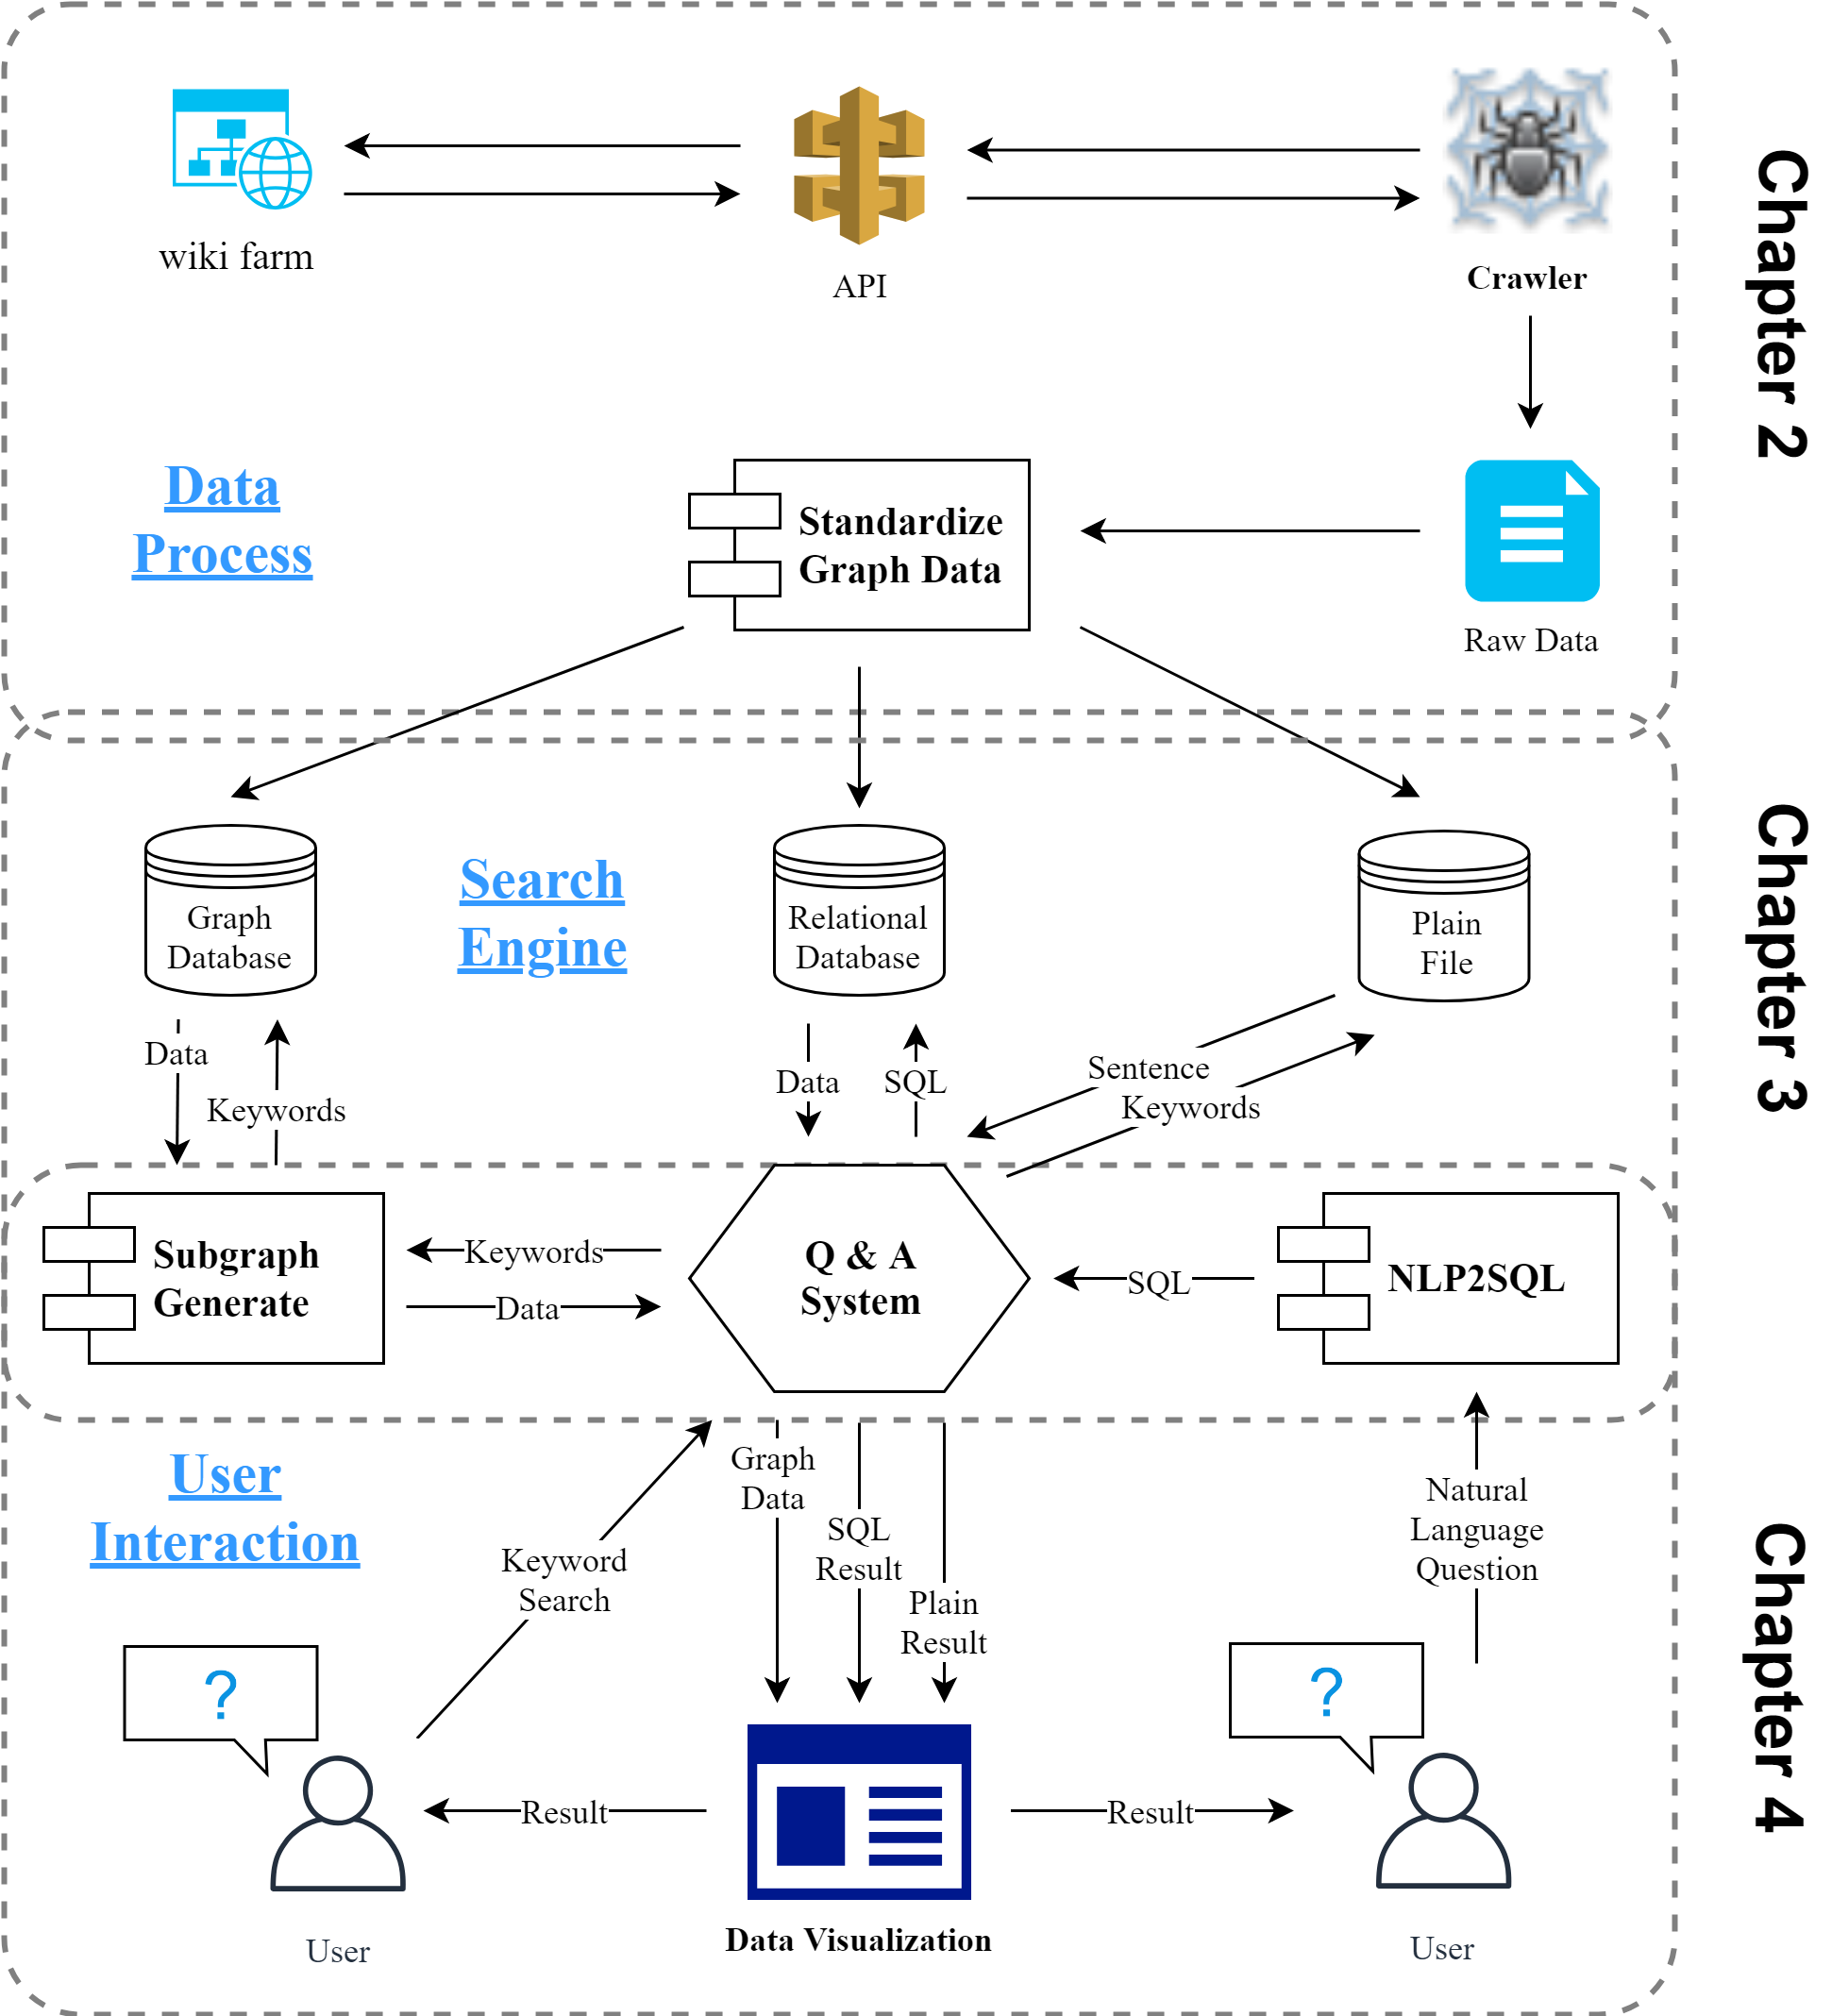
\includegraphics[width=1.05\linewidth]{fig/Section5.png}
\vspace{10pt}
\caption{The Structure of System Implementation}
\label{fig:section5-pic1}
\vspace{20pt}
\end{figure*}

\section{Visualization Technology}
\vspace{-5pt}
We use \href{https://plot.ly/}{Plotly}\footnote{https://plot.ly/} and \href{https://plot.ly/products/dash/}{Dash}\footnote{https://plot.ly/products/dash/} for the data visualization task. They are modern analytics applications which can build beautiful web-based interfaces in Python. \\
\indent At first, the project is built with Kivy and the plot function of igraph and the interface only loads the static figures. However, the interaction between these two packages can't realize what we desire. Different purposes with different builders influence their compatibility. It's hard to build a dynamic graph which can interact with users.\\ 
\indent Then, we decide to search for other tools to solve the data visualization tasks and choose the plotly instead. It can plot powerful, tidy, clean, dynamic graphs which meets our requirements, especially Scatter3d component. It is used for graph data plotting and user interaction. HTML components are used for listing text answers. Dropdown and input components are also used for user interaction.

\section{Implementation of Data Visualization}
\vspace{-5pt}
We set an input box on the main page and it has two modes. One is called Keyword Search, the other is called Fuzzy Search.\\
\indent In Keyword Search mode, the background program will find the articles and categories with similar characters to what user inputs. SEEKER will also return the plain file of the last keyword in the input box, and the text will print on the right side of the screen.\\
\indent In Fuzzy Search, the question that user types into the box will be sent to NLP2SQL module and translated into SQL query. After that, SEEKER will return the result and print it on the right side of the screen.\\
\indent In both cases, if there are keywords in the questions, the Subgraph Generate module will create a subgraph with keywords as its pivots, the relationships between keywords, categories and attributes of article keywords and their neighbors. Once the keywords change, the graph will regenerate immediately. 
